\documentclass[a4paper]{article}
\usepackage{amsmath}
%\usepackage[margin=3cm]{geometry}

\usepackage{graphicx}
\graphicspath{{../analysis/}{../../analysis/}{../static/}{../../static/}}

\usepackage[round]{natbib}
\bibliographystyle{unsrtnat}

\usepackage{url}

\newcommand{\hii}{H\textsc{ii}~}
\newcommand{\cloudy}{{\tt CLOUDY}~}

\title{The Physics of \hii Regions}\label{the-physics-of-hii-regions}
\author{Josh Borrow}

\begin{document}

\maketitle

\section{Introduction}

In this problem, we model the \hii region of an O star, within a cloud of
Hydrogen and Helium. It is worth starting with a brief description of what a
\hii region is, where they are found, and how they play a role. In Figure
\ref{fig:hiidiagram} we show a schematic of the ISM extracted from
\citet{borrow_towards_2017}.

\begin{figure}[!h]
    \centering
    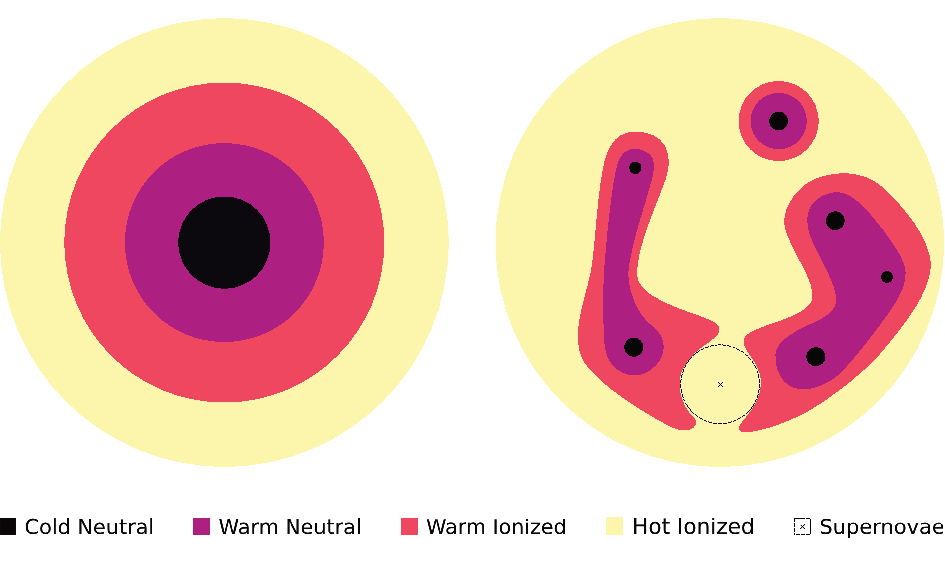
\includegraphics[width=\textwidth]{structure.pdf}
    \caption{The structure of the ISM. This is, in general, split up into four
        distinct parts in accordance with the work by
        \citet{mckee_theory_1977}.  The left image shows an isolated molecular
        cloud. The \hii region would correspond to the `ionised' regions around
        the central star forming `cold neutral' sphere. This is not the only
        time in which a \hii region forms, but in general they are found around
        collections of hot, young stars. Typically, a star will form in the
        cold neutral medium and ionise the region around it, forming an \hii
        region. On the right, a top-down image of the `large-scale' ISM is
        shown (around 1 kpc scale). It can be seen that multiple molecular
        clouds sit in the ISM, each surrounded by a large \hii region, full of
        newly-formed stars. Note that the \hii regions can be `joined'.}
    \label{fig:hiidiagram}
\end{figure}

\hii regions are associated with recent star formation
\citep{anderson_molecular_2009}, as is made clear by the schematic in Figure
\ref{fig:hiidiagram}.  They are formed primarily of ionised hydrogen, \hii, as
their name suggests, but are of course full of other ionised species as well,
such as He\textsc{ii}.  The temperature of these regions has been known to be
approximately $10^4$ K for many decades \citep{peimbert_temperature_1967}.

\section{Theoretical Study}

One of the first papers published on the theory behind \hii regions was by
\citet{stromgren_physical_1939}. Due to their relative abundance in the solar
neighborhood, \hii regions have been well studied; as far back as 
\citep{struve_emission_1938} it has been theorised that they arise due to
hot O and B stars that are present in regions of recent star formation.
In \citet{stromgren_physical_1939} the author makes the following key
assertions:
\begin{itemize}
    \item At the centre of the \hii region, there should be a collection of
          stars that produce ionising radiation.
    \item The photons from the star will ionise the gas around them. This
          gas will eventually re-combine, but this will emit a photon that is
          capable of ionising \emph{another} hydrogen atom (perhaps
          behind the original atom), ensuring that the `ionisation front'
          will always progress away from the star.
    \item The sphere should be fully ionised due to the large amount of
          ionising radiation produced by the star(s) and the aforementioned
          `back-propagation' mechanism.
    \item Eventually, the heating rate will be equal to the cooling rate
          (recombination rate) of the hydrogen nuclei, and at this point 
          the \hii region will end.
\end{itemize}
This leads naturally to the idea of a \citet{stromgren_physical_1939} sphere,
an ionised \hii region around a source of ionising photons. The sphere has
radius
\begin{align}
    R_S = \left(
    \frac{3}{4\pi} \frac{S_*}{n^2 \alpha} \right)^{1/3},
    \label{eqn:rs}
\end{align}
where $S_*$ is the luminosity of the central star in terms of photons per unit
time, $n$ is the number density of hydrogen in the cloud, and $\alpha
\approx 3\times 10^{-13}$ cm$^{4}$ s$^{-1}$ is the total recombination rate.
This is underlied by the following assumptions:
\begin{itemize}
    \item The density of hydrogen in the sphere is constant throughout, and
          the cloudy is composed solely of hydrogen.
    \item The number density of electrons in the sphere is the same as
          the number density of hydrogen nuclei.
    \item The sphere is fully ionised, and the boundary between the ionised
          region and the rest of the ISM is infinitely sharp (this can be shown
          to be true if the other assumptions also hold.
    \item The \hii region is at a constant temperature of ($10^{4}$ K).
\end{itemize})

In the section below, we will use the numerical radiative transfer code
\cloudy \citep{ferland_2017_2017} to assess if this theory produces
correct radii for \hii regions, and to interrogate the assumptions that the
above model makes.

\section{Numerical Study}

The \hii regions are now studied using the numerical radiative transfer code
\cloudy \citep{ferland_2017_2017}. In Table \ref{tab:sims} we list the
runs that were performed and hence what areas of parameter space were explored.

\begin{table}[!h]
    \centering
    \resizebox{\textwidth}{!}{
    \begin{tabular}{l|c|c|c|l}
        Run Name & Temperature (K) & Density ($n_H$ cm$^{-1}$) & $S_*$ & Abundances \\
        \hline
        {\tt dens\_var} & $35\times10^4$ & $10^1$ - $10^5$ & $10^{49}$ & ISM\\
        {\tt dens\_var\_only\_hydrogen} & $35\times10^4$ & $10^1$ - $10^5$ & $10^{49}$ & All $10^{-18}$ \\
        {\tt qh\_var} & $35\times10^4$ & $10^2$ & $10^{47}$ - $10^{52}$ & ISM\\
        {\tt temp\_var\_lowdensity} & $10$ - $100 \times 10^4$ & $10^1$ & $10^{49}$ & ISM \\
        {\tt temp\_var\_highdensity} & $10$ - $100 \times 10^4$ & $10^3$ & $10^{49}$ & ISM\\
    \end{tabular}}
    \caption{The runs presented below. Note that $S_*$ refers to the number of
        \emph{ionising} photons, i.e. this is {\tt q(h)} in the \cloudy code.}
    \label{tab:sims}
\end{table}
To compare our numerical runs with the theoretical predictions for the
\citet{stromgren_physical_1939} radius, we need to be able to extract the
cloud edge radius from from the simulation data. There are several ways to do
this, but here we choose to use the minimum of the derivative of the \hii
fraction (see Figure \ref{fig:derivative} for a pictorial version), as this
should be the turning point of the \hii curve. This will slightly
under-predict the cloud radius, but only if the transition between the cloud
and the rest of the ISM is not sharp. This turns out to be a reasonable
assumption for nearly all of the data collected (see figures below).

\begin{figure}[!h]
    \centering
    \includegraphics[width=\textwidth, trim=0.5cm 0.5cm 0.5cm 0.5cm]{differential.pdf}
    \caption{First derivatives of the H$\textsc{ii}$ abundance with respect to
        depth into cloud. The different lines correspond to different black
        body temperatures for the central star, at a fixed cloud density of
        $n_H = 1\times 10^3$. It is clear from Figure \ref{fig:density} that
        there is a turning point in the H$\textsc{ii}$ abundance at what
        appears to be the `edge' of the cloud. By using the minima of this
        derivative we can find the edge of the \hii region programmatically.}
    \label{fig:derivative}
\end{figure}

\subsection{Density}

As noted in Table \ref{tab:sims}, there are two sets of runs at various
abundances that are used to assess the scaling of the cloud radius with
hydrogen density. The first set are shown in Figure \ref{fig:density} and use
ISM abundances for species other than hydrogen in the cloud. This breaks the
assumption in \citet{stromgren_physical_1939} that the cloud is completely
composed of hydrogen, but we would still expect the abundances to be uniform
throughout the cloud, even though the density of electrons and nuclei may be
slightly diffrent. Another issue is that the different species will have
different ionisation energies, but as hydrogen is expected to be the most
dominant species, we can still assume that the stromgren radius should be a
\emph{upper} limit on the cloud radius. In this case, we would expect that the
cloud radius scales as $R_S \propto n^{-2/3}$, and this is shown in the final 
panel in the Figure \ref{fig:density}. However, we note that the cloud radius
scales much more strongly than this prediction.

\begin{figure}[!h]
\centering
\includegraphics[width=\textwidth, trim=1cm 1cm 1cm 0cm]{density_mixed.pdf}
    \caption{This plot shows the {\tt dens\_var} run.
        The hydrogen, H$\textsc{i}$, and H$\textsc{ii}$ densities are shown by
        the blue, orange, and green lines respectively. Note that the different
        panels correspond to varying initial hydrogen density. It is assumed
        that the cloud is equally dense throughout. The final panel shows how
        the radius of the H$\textsc{ii}$ and He$\textsc{ii}$ regions changes
        with cloud density.}
    \label{fig:density}
\end{figure}
In an attempt to disentagle effects of density change from the introduction
of other species, the {\tt dens\_var\_only\_hydrogen} run uses a very low
{\tt abundance = 1e-18} and the {\tt element limit off 0} command in \cloudy
to ensure that other species have no effect on the outcome of a run\footnote{
    it appears that this is the best/only way to do a hydrogen-only run in 
    \cloudy, but I am more than willing to be proved wrong}.
In Figure \ref{fig:densityhonly} we show the results from this run; these
are remarkably similar to the ones that are generated with all species present
at ISM abundances. We see the same scaling as before of cloud radius with
density (note that here the He\textsc{ii} line is not present due to a very
low helium fraction). This means that the difference in scaling must \emph{not}
be caused by interactions with different species giving the cloud a higher 
effective density due to changes in the interaction cross section.

\begin{figure}[!h]
\centering
\includegraphics[width=\textwidth, trim=1cm 1cm 1cm 0cm]{density_honly.pdf}
    \caption{This plot shows the {\tt dens\_var\_only\_hydrogen} run.
        The hydrogen, H$\textsc{i}$, and H$\textsc{ii}$ densities are shown by
        the blue, orange, and green lines respectively. Note that the different
        panels correspond to varying initial hydrogen density. It is assumed
        that the cloud is equally dense throughout. The final panel shows how
        the radius of the edge of the H$\textsc{ii}$ region changes with
        cloud density.}
    \label{fig:densityhonly}
\end{figure}
It is worth noting that in both of the density variation cases, at densities
greater than $\rho_H = 10^2$ cm$^{-3}$ we see a significant lack of ionisation
even before the cloud edge. This does not affect the scaling, however, as 
we even see similar scaling with density for the two fully-ionised points on
the final panel in both cases. It is also worth noting that \cloudy is a 1D
radiative transfer code, and this setup involves forcing it to run in pseudo-3D,
which may introduce some problems with various dimensional quantities. Here,
we see near-exact $1/n^2$ scaling with the density on cloud radius, as would
be expected in the 1D case; so it is very plausible that this is simply an
issue with the code or setup rather than an actual significant physical
difference.

\subsection{Temperature}\label{sec:temperature}

In the \cloudy paramterfile, we generally fix the number of ionising photons
that the central star emits. This means that by increasing the temperature,
we are lowering the luminosity overall, but increasing the luminosity in the
ionising frequency band, which is the region that will interact with our
cloud. We would expect, then, that this increased luminosity would increase
the temperature of the cloud (as is shown in Figure \ref{fig:cloudtemp}). It is
also important to note that in practice, even at a density of $n_H = 10^{3}$
cm$^{-3}$ the cloud is not fully ionised by a flux of $10^{49}$ $\gamma$
s$^{-1}$ (right panel of \ref{fig:cloudtemp}, see §\ref{sec:ionising}).

\begin{figure}[!h]
    \centering
    \includegraphics[width=0.49\textwidth, trim=0.5cm 0.5cm 0.5cm 0.5cm]{cloud_temp.pdf}
    \includegraphics[width=0.49\textwidth, trim=0.5cm 0.5cm 0.5cm 0.5cm]{cloud_ion.pdf}
    \caption{The cloud temperature as a function of stellar temperature (left),
        and the mean \hii fraction (right) in the {\tt temp\_var\_lowdensity}
        (the blue curve) and {\tt temp\_var\_highdensity} (the orange curve)
        runs averaged over the whole \hii region. We see similar scalings
        indepdendent of density for the temperature of the region, but a
        significant difference in the ionised fraction (see text).}
    \label{fig:cloudtemp}
\end{figure}
We would also expect that, if the cloud is not fully ionised, that the
ionisation fraction would increase as the temperature is increased due to an
overall higher luminosity of ionising photons. This turns out not to be the
case, as is shown in the right panel of Figure \ref{fig:cloudtemp}. It is
possible that this is due to a change in the mean energy of the ionising
photons; the ionisation cross-section for H\textsc{i} drops with increasing
photon energy \citep{palenius_absolute_1976}. This would mean that more
photons would be escaping the cloud without interacting with any hydrogen
atoms (an effective drop in $S_*$). 

\begin{figure}[!h]
    \centering
    \includegraphics[width=\textwidth, trim=1cm 1cm 1cm 0.5cm]{lowdensity.pdf}
    \caption{The different panels correspond to different central star
        temperatures. {\tt temp\_var\_lowdensity} Note that each of these
        panels has a fixed $S_* = 10^{49}$ ionising photons per second
        luminosity. The final panel shows the convergence to the stromgren
        radius for a very hot star, where the photons in general are more
        energetic. The quick rise at low temperatures for He\textsc{ii} is due to
        the very high ionisation potential for helium; see text.}
    \label{fig:templowdens}
\end{figure}
In Figure \ref{fig:templowdens} we show the {\tt temp\_var\_lowdensity} runs.
note that we see much better convergence to the theoretical
\citet{stromgren_physical_1939} radius than in the density variation case.
This lends credence to the theory that issues in convergence for the density
variation case is due to code or setup errors, as here we perform an effective
`null' test; we expect no change in the radius of the cloud. Changes in cloud
radius can be explained through the above mentioned ionisation cross-section
and changes in the luminosity. As the stellar temperature is increased, more
photons are above the 24.6 eV threshold to produce He\textsc{ii}, leading to
the steady increase in `He\textsc{ii}' cloud radius. In this low density test,
we see that the \hii region should be almost fully ionised (Figure
\ref{fig:cloudtemp}), and hence there is very little scaling of the \hii
cloud radius with temperature due to the fixed number ($S_* = 10^{49}$) of
ionising photons.

\subsection{Ionising Radiation Flux}\label{sec:ionising}

In this section we vary {\tt q(h)} = $S_*$ the number of ionisng photons
produced per second by the star; see Figure \ref{fig:qhvar} for the results.
In this case, where $n_H = 10^2$ cm$^{-3}$ and $T_{\rm star} = 35000$ K remain
fixed, we see that only above $S_* = 10^{49}$ does the cloud become fully
ionised. Unlike §\ref{sec:temperature} here \emph{both} the luminosity of the
star and the luminosity in the ionising band increases, and hence the
ionisation cross section for hydrogen at high energies has less of an effect.
the mean ionisation fraction as previously. As expected, with increasing
$S_*$ the cloud radius increases.

\begin{figure}
    \centering
    \includegraphics[width=\textwidth, trim=1cm 1cm 1cm 0.5cm]{qh_var.pdf}
    \caption{This figure shows the results from the {\tt qh\_var} run. Note
        again the stronger than expected scaling of the cloud radius with
        $S_*$; this scaling is exactly $R_S \propto S_*$ rather than
        $R_S \propto S_*^{1/3}$. This again lends credence to the idea that
        there was some issue with code setup leading to an effectively
        1D problem being ran.}
    \label{fig:qhvar}
\end{figure}

\section{Discussion}

In this work we have shown using \cloudy that:
\begin{itemize}
    \item We see broadly the same changes in cloud radius as is expected
          from the \citet{stromgren_physical_1939} sphere when the density,
          temperature, and ionising photon flux is changed.
    \item The assumption that the cloud changes rapidly from a fully-ionised
          state to a neutral state is invalid when the cloud itself is not
          completely ionised (the mean \hii fraction is about 0.9).
    \item The temperature of the star plays a significant role in the dynamics
          of the cloud structure, as well as the ionisation fraction; this is
          due to a dependence on energy in the hydrogen ionisation
          cross-section.
    \item In general, the \citet{stromgren_physical_1939} radius provides an
          \emph{upper} limit on the cloud radius, due to other cooling
          processes and species inside the cloud `eating' more photons than
          was originally assumed.
\end{itemize}

\section{Codes}

You can find all of the codes, parameterfiles, and even the \LaTeX~ source
for this report in the following GitHub repository,\\
\url{https://github.com/JBorrow/cloudy-hii-regions-homework}.

\bibliography{library}

\end{document}
